% Block 3 of lista-reais-lectures-01-05 (input by the drivers in Listas/).
% Order and ratings: lista-reais-lectures-01-05/order.md.
\bloco{3}{Dynamic games: extensive form, backward induction, SPE}{Lecture 3}

% ---------------------------------------------------------------------------
\exercicio[1]{Strategies}{Foundations}{Tadelis (2013), \emph{Game Theory: An Introduction}, Ch.~7
``Preliminaries'', Exercise 7.1 ``Strategies'', p.~147 [PDF 166]. No answer in the book.
Reproduced verbatim.}

\rot{7.1}\textbf{Strategies:} Imagine an extensive-form game in which player $i$ has $K$ information
sets.
\begin{partes}
\item If the player has an identical number of $m$ possible actions in each information set, how
many pure strategies does he have?
\item If the player has $m_k$ actions in information set $k \in \{1, 2, \ldots, K\}$, how many pure
strategies does the player have?
\end{partes}
\resolespaco

% ---------------------------------------------------------------------------
\exercicio[1]{Sequential Version of the Prisoner's Dilemma Game}{Foundations}{Muñoz-Garcia \&
Toro-Gonzalez (2019), \emph{Strategy and Game Theory: Practice Exercises with Answers}, 2nd ed.,
Ch.~4 ``Sequential-Move Games with Complete Information'', Exercise 3 ``Sequential Version of the
Prisoner's Dilemma Game''$^{\mathrm{A}}$, p.~160 [PDF 172]. Worked answer in the book, right after
the statement. Reproduced verbatim (statement only); Fig.~4.9 cropped from the page.}

Consider the game tree in Fig.~4.9, representing the sequential-move version of the Prisoner's
dilemma game, where player 1 acts first, and observing its move player 2 responds.
\begin{center}
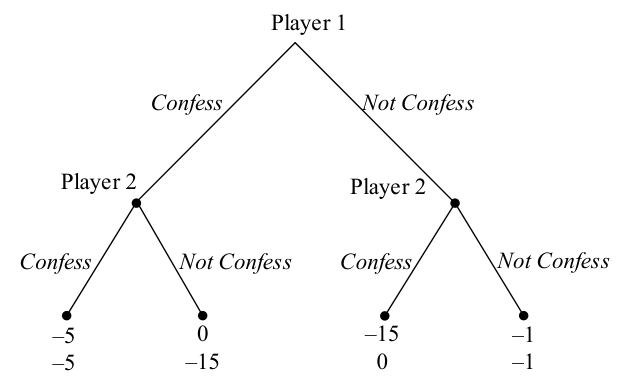
\includegraphics[width=0.55\linewidth]{figures/munoz-garcia-4-3.png}\\[2pt]
\small\textit{Fig.~4.9} Prisoner's dilemma sequential-move game
\end{center}
\begin{enumerate}[label=(\alph*),leftmargin=2em]
\item Find the best responses of the second mover, for each of the first mover's actions.
\item Find the first mover's equilibrium action and describe the subgame perfect Nash equilibrium of
the game.
\item Does the equilibrium behavior in the sequential-move game differ from its simultaneous-move
version?
\end{enumerate}

\begin{referencia}{``its simultaneous-move version'': Muñoz-Garcia \& Toro-Gonzalez (2019), Ch.~1,
Exercise 5 ``Prisoners' Dilemma Game'', Fig.~1.8, p.~9 [PDF 22]. Matrix rebuilt from the page.}
\jogo{Prisoner 1}{Prisoner 2}{\begin{tabular}{c|c|c|}
\hd{} & \hd{Confess} & \hd{Not confess}\\\cline{2-3}
Confess & -5, -5 & 0, -15\\\cline{2-3}
Not confess & -15, 0 & -1, -1\\\cline{2-3}
\end{tabular}}
\vspace{-6pt}\begin{center}\textit{Fig.~1.8} Normal-form of Prisoners' dilemma game\end{center}
\end{referencia}
\resolespaco

% ---------------------------------------------------------------------------
\exercicio[2]{Strategies and Equilibrium}{Foundations}{Tadelis (2013), \emph{Game Theory: An
Introduction}, Ch.~7 ``Preliminaries'', Exercise 7.2 ``Strategies and Equilibrium'', p.~147 [PDF
166]. No answer in the book. Reproduced verbatim.}

\rot{7.2}\textbf{Strategies and Equilibrium:} Consider a two-player game in which player 1 can
choose $A$ or $B$. The game ends if he chooses $A$ while it continues to player 2 if he chooses
$B$. Player 2 can then choose $C$ or $D$, with the game ending after $C$ and continuing again with
player 1 after $D$. Player 1 can then choose $E$ or $F$, and the game ends after each of these
choices.
\begin{partes}
\item Model this as an extensive-form game tree. Is it a game of perfect or imperfect information?
\item How many terminal nodes does the game have? How many information sets?
\item How many pure strategies does each player have?
\item Imagine that the payoffs following choice $A$ by player 1 are $(2, 0)$, those following $C$ by
player 2 are $(3, 1)$, those following $E$ by player 1 are $(0, 0)$, and those following $F$ by
player 1 are $(1, 2)$. What are the Nash equilibria of this game? Does one strike you as more
``appealing'' than the other? If so, explain why.
\end{partes}
\resolespaco

% ---------------------------------------------------------------------------
\exercicio[3]{Technology Adoption}{Exam level}{Tadelis (2013), \emph{Game Theory: An Introduction},
Ch.~8 ``Credibility and Sequential Rationality'', Exercise 8.5 ``Technology Adoption'', p.~170 [PDF
189]. No answer in the book. Reproduced verbatim.}

\rot{8.5}\textbf{Technology Adoption:} During the adoption of a new technology a CEO (player 1) can
design a new task for a division manager. The new task can be either high level ($H$) or low level
($L$). The manager simultaneously chooses to invest in good training ($G$) or bad training ($B$).
The payoffs from this interaction are given by the following matrix:
\jogo{Player 1}{Player 2}{\begin{tabular}{c|c|c|}
\hd{} & \hd{$G$} & \hd{$B$}\\\cline{2-3}
$H$ & 5, 4 & $-5$, 2\\\cline{2-3}
$L$ & 2, $-2$ & 0, 0\\\cline{2-3}
\end{tabular}}
\begin{partes}
\item Present the game in extensive form (a game tree) and solve for all the Nash equilibria and
subgame-perfect equilibria.
\item Now assume that before the game is played the CEO can choose not to adopt this new technology,
in which case the payoffs are (1, 1), or to adopt it, in which case the game is played. Present the
\emph{entire} game in extensive form. How many proper subgames does it have?
\item Solve for all the Nash equilibria and subgame-perfect equilibria of the game described in (b).
\end{partes}
\resolespaco

% ---------------------------------------------------------------------------
\exercicio[3]{Playing It Safe}{Exam level}{Tadelis (2013), \emph{Game Theory: An Introduction}, Ch.~8
``Credibility and Sequential Rationality'', Exercise 8.10 ``Playing It Safe'', p.~172 [PDF 191]. No
answer in the book. Reproduced verbatim.}

\rot{8.10}\textbf{Playing It Safe:} Consider the following dynamic game: Player 1 can choose to play
it safe (denote this choice by $S$), in which case both he and player 2 get a payoff of 3 each, or he
can risk playing a game with player 2 (denote this choice by $R$). If he chooses $R$ then they play
the following simultaneous-move game:
\jogo{Player 1}{Player 2}{\begin{tabular}{c|c|c|}
\hd{} & \hd{$A$} & \hd{$B$}\\\cline{2-3}
$C$ & 8, 0 & 0, 2\\\cline{2-3}
$D$ & 6, 6 & 2, 2\\\cline{2-3}
\end{tabular}}
\begin{partes}
\item Draw a game tree that represents this game. How many proper subgames does it have?
\item Are there other game trees that would work? Explain briefly.
\item Construct the matrix representation of the normal form of this dynamic game.
\item Find all the Nash and subgame-perfect equilibria of the dynamic game.
\end{partes}
\resolespaco

% ---------------------------------------------------------------------------
\exercicio[3]{Centipedes}{Exam level}{Tadelis (2013), \emph{Game Theory: An Introduction}, Ch.~7
``Preliminaries'', Exercise 7.4 ``Centipedes'', p.~148 [PDF 167]. No answer in the book.
Reproduced verbatim.}

\rot{7.4}\textbf{Centipedes:} Imagine a two-player game that proceeds as follows. A pot of money is
created with \$6 in it initially. Player 1 moves first, then player 2, then player 1 again, and
finally player 2 again. At each player's turn to move, he has two possible actions: grab ($G$) or
share ($S$). If he grabs he gets $\frac{2}{3}$ of the current pot of money, the other player gets
$\frac{1}{3}$ of the pot, and the game ends. If he shares then the size of the current pot is
multiplied by $\frac{3}{2}$ and the next player gets to move. At the last stage at which player 2
moves, if he chooses $S$ then the pot is still multiplied by $\frac{3}{2}$, player 2 gets
$\frac{1}{3}$ of the pot, and player 1 gets $\frac{2}{3}$ of the pot.
\begin{partes}
\item Model this as an extensive-form game tree. Is it a game of perfect or imperfect information?
\item How many terminal nodes does the game have? How many information sets?
\item How many pure strategies does each player have?
\item Find the Nash equilibria of this game. How many outcomes can be supported in equilibrium?
\item Now imagine that at the last stage at which player 2 moves, if he chooses to share then the
pot is equally split among the players. Does your answer to part (d) change?
\end{partes}
\resolespaco

% ---------------------------------------------------------------------------
\exercicio[4]{The Dean's Dilemma}{Exam level}{Tadelis (2013), \emph{Game Theory: An Introduction},
Ch.~7 ``Preliminaries'', Exercise 7.9 ``The Dean's Dilemma'', pp.~149--150 [PDF 168--169]. No
answer in the book. Reproduced verbatim.}

\rot{7.9}\textbf{The Dean's Dilemma:} A student stole the DVD player from the student lounge. The dean
of students (player 1) suspects the student (player 2) and begins collecting evidence. However,
evidence collection is a random process, and concrete evidence will be available to the dean only
with probability $\frac{1}{2}$. The student knows that the evidence-gathering process is under way
but does not know whether the dean has collected evidence or not. The game proceeds as follows: The
dean realizes whether or not he has evidence and can then choose his action, whether to accuse the
student ($A$) or bounce the case ($B$) and forget it. Once accused, the student has two options: he
can either confess ($C$) or deny ($D$). Payoffs are realized as follows: If the dean bounces the case
then both players get 0. If the dean accuses the student and the student confesses, the dean gains
2 and the student loses 2. If the dean accuses the student and the student denies, then payoffs
depend on the evidence: If the dean has no evidence then he loses face, which gives him a loss of
4, while the student gains glory, which gives him a payoff of 4. If, however, the dean has evidence
then he is triumphant and gains 4, while the student is put on probation and loses 4.
\begin{partes}
\item Draw the game tree that represents the extensive form of this game.
\item Write down the matrix that represents the normal form of the extensive form you drew in (a).
\item Solve for the Nash equilibria of the game.
\end{partes}
\resolespaco

% ---------------------------------------------------------------------------
\exercicio[4]{Perfect and Imperfect Recall}{Exam level}{Tadelis (2013), \emph{Game Theory: An
Introduction}, Ch.~7 ``Preliminaries'', Exercise 7.10 ``Perfect and Imperfect Recall'', p.~150 [PDF
169]. No answer in the book. Reproduced verbatim; Figure 7.14 cropped from the page.}

\rot{7.10}\textbf{Perfect and Imperfect Recall:} Consider the game depicted in Figure 7.14.
\begin{center}
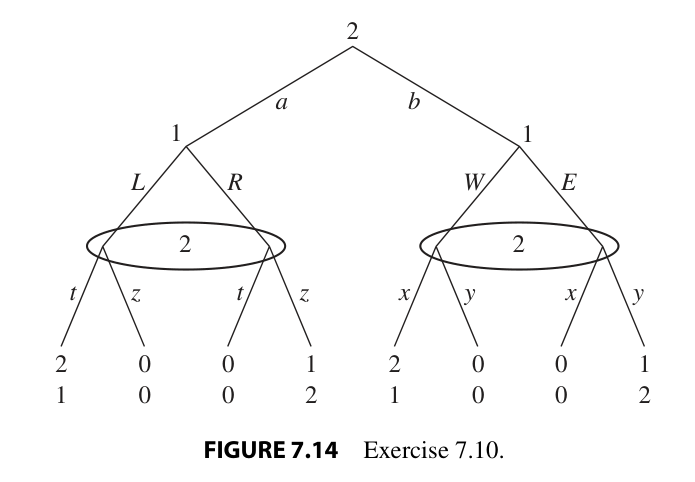
\includegraphics[width=0.6\linewidth]{figures/tadelis-7-10.png}
\end{center}
\begin{partes}
\item What are the pure-strategy sets for each player?
\item Show that for any behavioral strategy for player 1 there is a mixed strategy that leads to the
same distribution over the terminal nodes regardless of the strategy chosen by player 2.
\item Show that for any behavioral strategy for player 2 there is a mixed strategy that leads to the
same distribution over the terminal nodes regardless of the strategy chosen by player 1.
\item Now imagine that the game does not have perfect recall so that player 2's bottom two
information sets are now one large information set. Can you find an example showing that the claim
in (c) is no longer true?
\end{partes}
\resolespaco

% ---------------------------------------------------------------------------
\exercicio[4]{Zero-sum games of perfect information}{Advanced}{Mas-Colell, Whinston \& Green (1995),
\emph{Microeconomic Theory}, Ch.~9 ``Dynamic Games'', Exercises, Exercise 9.B.4$^{\mathrm{B}}$,
p.~302 [PDF 162, left half]. Answer in the MWG solutions manual (\texttt{Livros/}). Reproduced
verbatim.}

\rot{9.B.4$^{\mathrm{B}}$}Prove that in a finite \emph{zero-sum} game of perfect information, there
are unique subgame perfect Nash equilibrium payoffs.
\resolespaco

% ---------------------------------------------------------------------------
\exercicio[5]{The Rotten Kid Theorem}{Advanced}{Gibbons (1992), \emph{Game Theory for Applied
Economists}, Ch.~2 ``Dynamic Games of Complete Information'', \S2.6 Problems (Section 2.1),
Problem 2.1, p.~130 [PDF 137]. No answer in the book. Reproduced verbatim.}

\rot{2.1.}Suppose a parent and child play the following game, first analyzed by Becker (1974).
First, the child takes an action, $A$, that produces income for the child, $I_C(A)$, and income for
the parent, $I_P(A)$. (Think of $I_C(A)$ as the child's income net of any costs of the action $A$.)
Second, the parent observes the incomes $I_C$ and $I_P$ and then chooses a bequest, $B$, to leave to
the child. The child's payoff is $U(I_C + B)$; the parent's is $V(I_P - B) + kU(I_C + B)$, where
$k > 0$ reflects the parent's concern for the child's well-being. Assume that: the action is a
nonnegative number, $A \ge 0$; the income functions $I_C(A)$ and $I_P(A)$ are strictly concave and
are maximized at $A_C > 0$ and $A_P > 0$, respectively; the bequest $B$ can be positive or negative;
and the utility functions $U$ and $V$ are increasing and strictly concave. Prove the ``Rotten Kid''
Theorem: in the backwards-induction outcome, the child chooses the action that maximizes the
family's aggregate income, $I_C(A) + I_P(A)$, even though only the parent's payoff exhibits
altruism.
\resolespaco
